\documentclass{article}
\usepackage{xeCJK,amsmath,geometry,float,graphicx,amssymb,zhnumber,booktabs,setspace,tasks,verbatim,amsthm,amsfonts,mathdots}
\usepackage{listings,xcolor,diagbox}
\geometry{a4paper,scale=0.8}  
\renewcommand\arraystretch{2}
\title{图论作业 (Week 13)}
\author{PB20000113孔浩宇}
\begin{document}
\maketitle
\section*{Ch9}
\subsection*{1.}
\begin{proof}
    $\forall\ e=(v,u)\in E(D),\ e\in \alpha(v),\ e\in \beta(u) $,有
    \[
        \sum\limits_{v\in V(D)} \sum\limits_{e\in \alpha(v)} f(e)
        =
        \sum\limits_{u\in V(D)} \sum\limits_{e\in \beta(u)} f(e)
    \]
    又$\forall\ v\in V(D)-\{s,t\},\ \sum\limits_{e\in \alpha(v)} f(e) = \sum\limits_{e\in \beta(v)} f(e)$,可联立解得
    \[
        \sum\limits_{e\in \alpha(s)} f(e) + \sum\limits_{e\in \alpha(t)} f(e)
        =
        \sum\limits_{e\in \beta(s)} f(e) + \sum\limits_{e\in \beta(t)} f(e)
    \]
    即
    \[
        \sum\limits_{e\in \alpha(t)} f(e) - \sum\limits_{e\in \beta(t)} f(e)
        =
        \sum\limits_{e\in \beta(s)} f(e) - \sum\limits_{e\in \alpha(s)} f(e)
    \]
\end{proof}

\subsection*{2.}
\begin{proof}
    \begin{enumerate}
        \item []
        \item [(1)]首先证$\forall\ e\in E(D)$,有$c(e) \geq \overline{f} (e) \geq 0$.
        \begin{enumerate}
            \item [(a)]$e\notin P(s,t)$.
            \[
                c(e)\geq f(e) = \overline{f}(e) \geq 0
            \]
            \item [(b)]$e$为正向边
            \[
                c(e)=f(e) + c(e) - f(e)
                \geq f(e) + l(P)
                = \overline{f} (e)
                \geq 0
            \]
            \item [(c)]$e$为反向边
            \[
                c(e)\geq f(e)
                > f(e) - l(P)
                \geq 0
            \]
        \end{enumerate}
        \item [(2)]再证$\forall\ v\in V(D)-\{s,t\}$,都有$\sum\limits_{e\in \alpha(v)} \overline{f} (e) - \sum\limits_{e\in \beta(v)} \overline{f}(e)=0$.
        \begin{enumerate}
            \item [(a)]$v\notin P(s,t)$.此时
            \[
                \forall\ e\in \alpha(v)\mbox{或} e\in \beta(v),\ 
                \overline{f}(e) = f(e)\ 
                \Rightarrow\ 
                \sum\limits_{e\in \alpha(v)} \overline{f}(e) - \sum\limits_{e\in \beta(v)}\overline{f}(e)=
                \sum\limits_{e\in \alpha(v)} f(e) - \sum\limits_{e\in \beta(v)}f(e)=0
            \]
            \item [(b)]$v\in P(s,t)$.不妨设$P(s,t)=s\cdots e_1 v e_2 \cdots t$.取$e_1, e_2$均为正向边的情况.
            \begin{align*}
                &\sum\limits_{e\in\alpha (v)} \overline{f}(e) - \sum\limits_{e\in \beta (v)} \overline{f}(e) \\
                =&\left[\overline{f}(e_1) + \sum\limits_{e\in\alpha (v)- \{e_1\} } \overline{f}(e) \right]
                - \left[\overline{f}(e_2) + \sum\limits_{e\in\beta (v)- \{e_2\} } \overline{f}(e) \right]\\
                =&\left[l(P) + f(e_1) + \sum\limits_{e\in\alpha (v)- \{e_1\} } f(e) \right]
                - \left[l(P) + f(e_2) + \sum\limits_{e\in\beta (v)- \{e_2\} } f(e) \right]\\
                =&\sum\limits_{e\in \alpha(v)} f(e) - \sum\limits_{e\in \beta(v)}f(e)\\
                =&0.
            \end{align*}
            其余情况同理可得.
        \end{enumerate}
    \end{enumerate}
\end{proof}

\subsection*{4.}
\begin{enumerate}
    \item [(1)]取初始流$f\equiv 0$.
    \item [(2)]找到可增载轨道$u v_1 v_3 v_4 t$,此时$l(P)=3$,有修正后流函数
    
    \begin{figure*}[htbp]
        \centering
        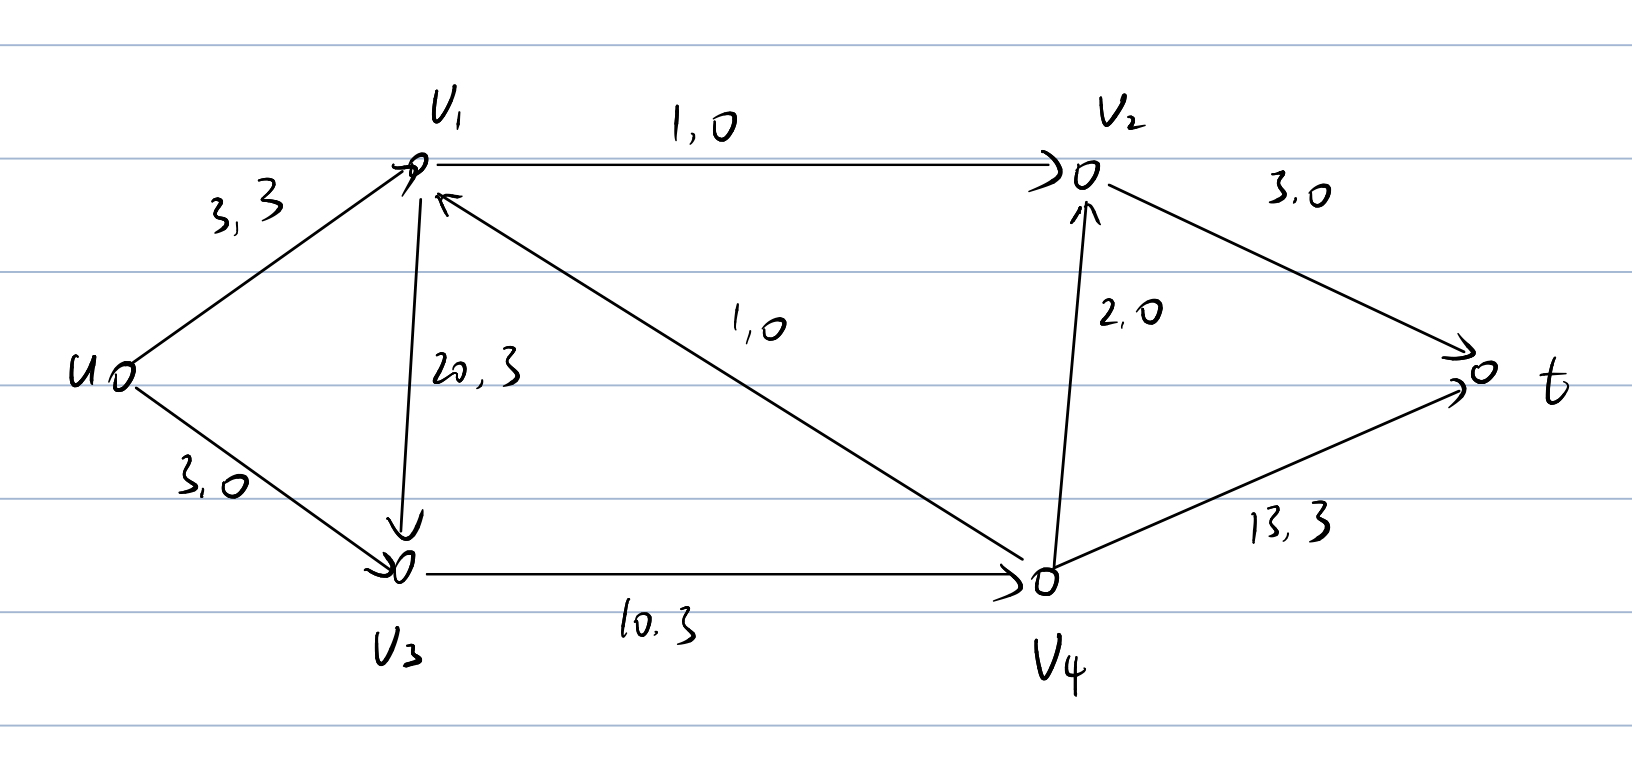
\includegraphics[scale=0.2]{42.PNG}
    \end{figure*}

    \item [(3)]找到可增载轨道$u v_3 v_4 t$,此时$l(P)=3$,有修正后流函数
    \begin{figure*}[htbp]
        \centering
        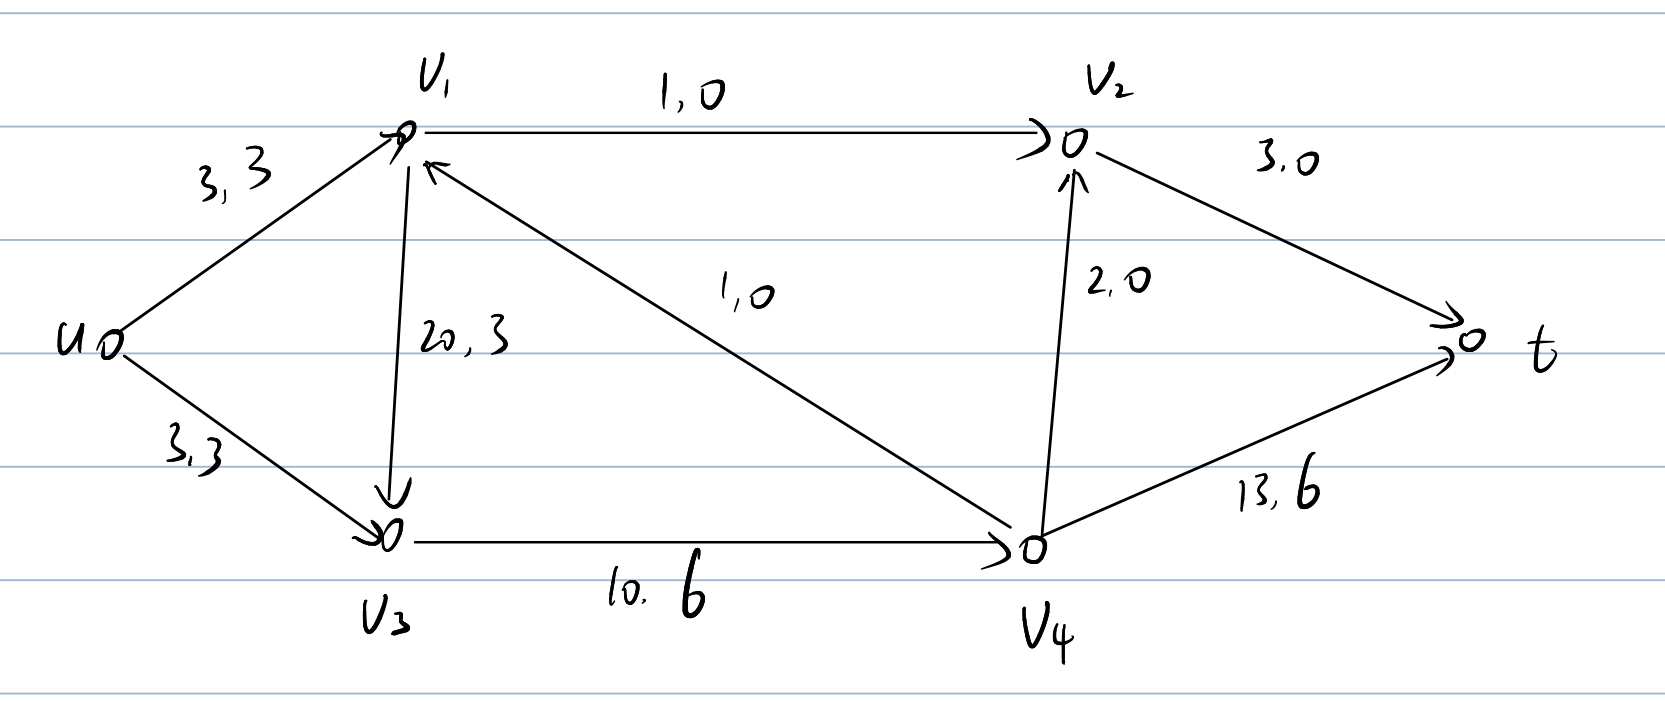
\includegraphics[scale=0.2]{43.PNG}
    \end{figure*}

    \item [(4)]无可增载轨道,最大流为6.
\end{enumerate}

\subsection*{5.}
\begin{proof}
    对于任意的截,
    \[
        C(S,\bar{S})=\sum_{e\in (S,\bar{S})c}c(e)
        \ \Rightarrow\ 
        C(S,\bar{S})\mbox{为整数,因此最小截也为整数.}
    \]

    由因为最大流最小截定理,最大流等于最小截,故最大流也一定是整数。
\end{proof}

\subsection*{7.}
    如图
    \begin{figure*}[htbp]
        \centering
        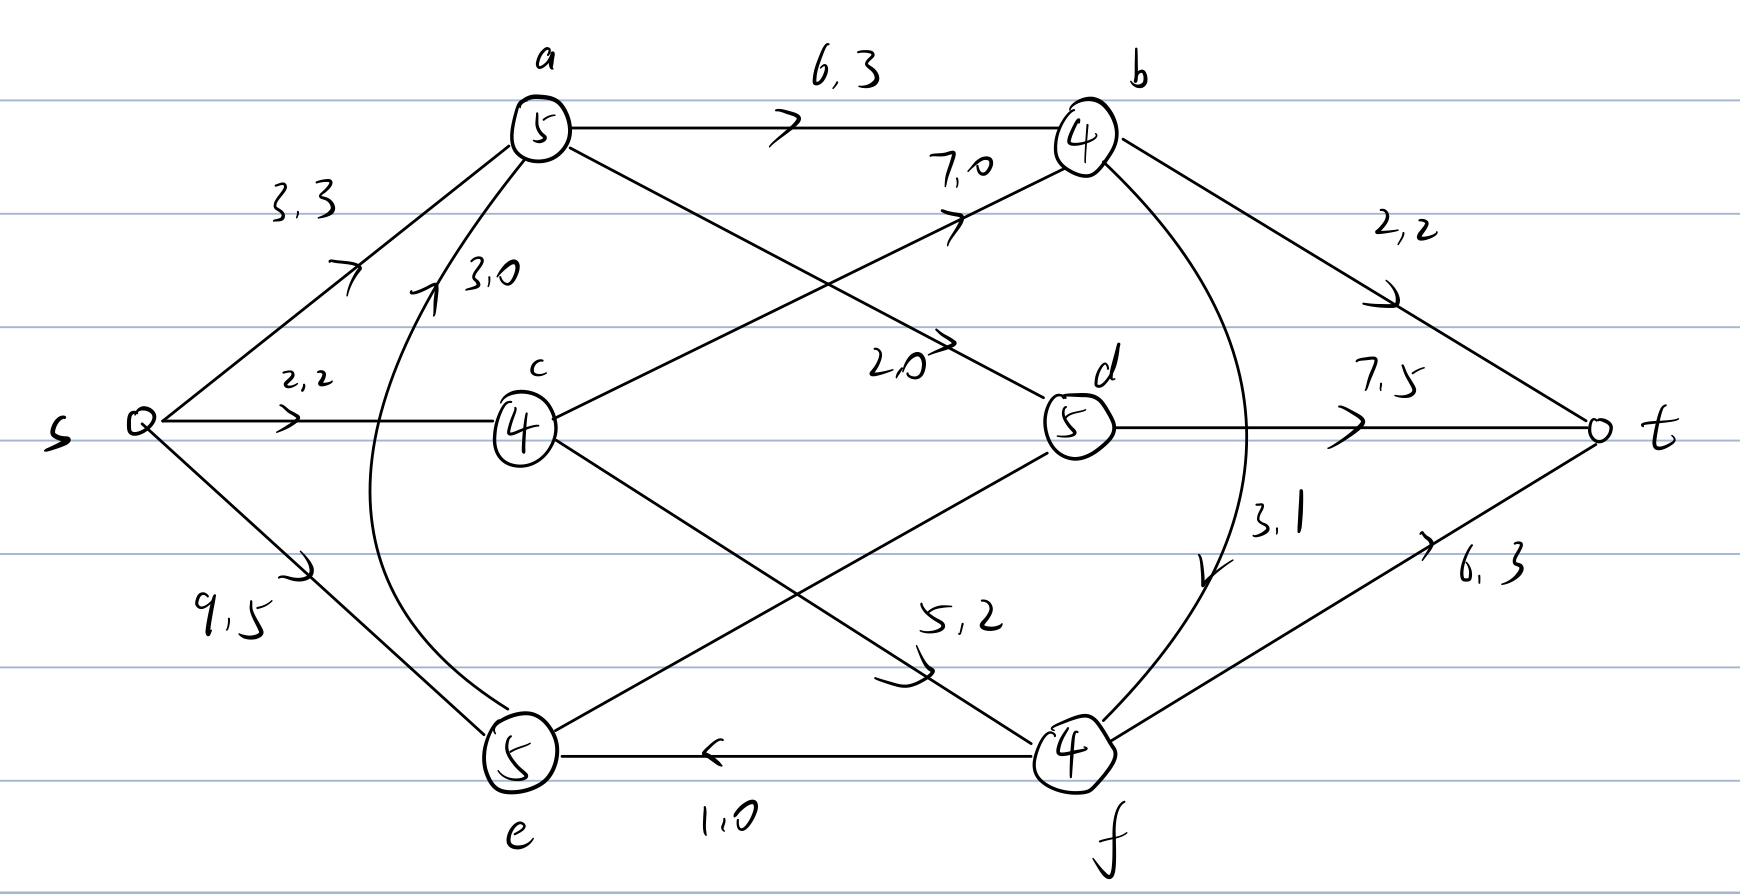
\includegraphics[scale=0.2]{7.PNG}
    \end{figure*}

\subsection*{10.}
\begin{proof}
    \begin{align*}
        D\mbox{有可行流}& \Leftrightarrow \mbox{伴随网络}N\mbox{的最大流使}\forall\ e\in V\mbox{都满载}
    \end{align*}
\end{proof}

\subsection*{13.}
    不存在可行流,$\{c\}$需漏掉流,$\{d\}$需冒出流。

\end{document}